\documentclass[UTF8,zihao=-4,fontset=windows]{ctexart}

\usepackage[a4paper,left=2.5cm,right=2.5cm,top=2.5cm,bottom=2.5cm]{geometry}
\usepackage{graphicx}
\usepackage{booktabs}
\usepackage{tabularx}
\usepackage{array}
\usepackage{float}
\usepackage{caption}
\usepackage{setspace}
\usepackage{hyperref}
\usepackage{xcolor}
\usepackage{enumitem}
\usepackage{xurl}

\graphicspath{{assets/}}
\captionsetup{font=small,labelfont=bf,labelsep=quad}
\hypersetup{colorlinks=true,linkcolor=black,urlcolor=blue,citecolor=black}
\setstretch{1.35}
\setlist{nosep,leftmargin=2em}

\newcommand{\blankline}[1]{\makebox[#1]{\hrulefill}}
\newcommand{\reporttitle}{数据可视化视角下的中证2000成分股画像分析}

\begin{document}

\begin{titlepage}
  \centering
  \vspace*{1.5cm}
  {\zihao{2}\bfseries 《数据可视化》课程论文/报告\par}
  \vspace{0.5cm}
  {\zihao{4}(2025--2026学年第2学期)\par}
  \vspace{2.2cm}

  {\zihao{3}\bfseries 题目\quad \reporttitle\par}
  \vspace{2.2cm}

  \begin{tabular}{>{\zihao{-4}}r >{\zihao{-4}}l}
    学生姓名 & \blankline{7cm} \\[0.9cm]
    学号 & \blankline{7cm} \\[0.9cm]
    提交日期 & 2026年6月20日 \\[0.9cm]
  \end{tabular}

  \vspace{1.3cm}
  \renewcommand{\arraystretch}{1.8}
  \begin{tabularx}{0.88\textwidth}{|>{\centering\arraybackslash}p{3cm}|X|>{\centering\arraybackslash}p{3cm}|X|}
    \hline
    上课时间 & & QQ/手机 & \\
    \hline
    所在学院 & & 专业 & \\
    \hline
  \end{tabularx}

  \vspace{1.3cm}
  \begin{tabularx}{0.88\textwidth}{|>{\centering\arraybackslash}p{3cm}|X|}
    \hline
    教师评语 & \vspace{4.2cm} \\
    \hline
    本论文成绩评定 & \blankline{4cm}\quad 分 \\
    \hline
  \end{tabularx}

  \vfill
\end{titlepage}

\begin{center}
  {\zihao{3}\bfseries \reporttitle}
\end{center}

\section*{摘要}
我们以中证2000成分股为研究对象，分析2026年1月5日至2026年5月29日的市场行情数据，构建面向中小市值股票画像的数据可视化框架。样本包含2,000只成分股、189,811条个股日线记录和95条指数日线记录。我们先将个股行情整理为可比较的时间序列与横截面数据，再围绕价格、成交量、成交额、涨跌幅和换手率等字段进行异常识别、缺失处理与指标重组，并从收益、风险、量价关系、形态特征和交易活跃度等方面提取29个股票级特征。基于标准化特征进行主成分分析和 KMeans 聚类后，11个主成分解释90.87\%的特征方差，轮廓系数支持3类股票画像结构。

可视化结果揭示了指数走势与个股分化之间的差异。指数走势、涨跌家数和成交额图刻画市场阶段变化；月度收益分布、累计收益排名、波动率和最大回撤图呈现风险收益结构；换手率、涨跌停次数和价量相关系数图补充交易行为证据；PCA 散点图、雷达图和代表股走势图进一步解释股票类型差异。样本期内中证2000整体经历震荡上行、阶段回撤和反弹修复，但个股截面分化显著。放量突破型股票数量较少但平均收益最高，高弹性反弹型股票具有更强价格弹性和更高回撤风险，低流动性型股票数量最多且平均收益偏弱。结果表明，中小市值股票池的市场表现不能仅由指数点位解释，需要结合风险、流动性、量价结构和聚类画像进行多维观察。

\noindent\textbf{关键词}\quad 数据可视化；中证2000；金融时间序列；PCA；KMeans；股票画像

\section{引言}
股票市场数据同时包含时间变化和横截面差异，单一指数曲线只能概括市场方向，难以解释个股之间的收益分化、风险暴露和交易活跃度差异。数据可视化的价值在于把密集数据转化为可观察、可比较的图形结构，使分析者能够在趋势、分布、关系和分组之间建立联系。Cleveland 和 McGill 将图形感知视为从图形编码中解读定量和定性信息的过程，这一观点提示图表设计不仅影响结果呈现，也影响读者对数据结构的判断。Shneiderman 提出的信息寻求思路强调先观察整体，再筛选局部，最后进入细节。该思路适用于金融市场画像分析，因为股票池规模较大，直接进入个股细节容易忽略整体结构，只停留在指数层面又会遮蔽微观差异。

中证2000指数选取市值规模较小且流动性较好的2,000只证券作为样本，与沪深300、中证500和中证1000共同构成中证规模指数系列。该指数适合观察中小市值股票的整体表现和内部结构。与大盘蓝筹指数相比，中小市值股票通常具有更强的交易弹性和更明显的个股分化，其走势受流动性、主题轮动、风险偏好和短期资金行为影响较大。对这类股票池进行可视化分析，关键不只是画出指数涨跌，而是同时处理宏观市场环境和微观个体差异。

我们围绕中证2000成分股构建多层次图表体系，重点回答三个问题。第一，2026年1月至5月中证2000总体经历了怎样的市场阶段。第二，成分股在收益、波动、回撤和交易行为上呈现哪些横截面差异。第三，基于多维特征能否形成具有解释意义的股票画像。研究不以短期预测为主要目标，而是通过数据处理和图表表达揭示股票池内部结构，使市场现象、统计特征和典型个股之间形成相互印证的分析链条。

\section{数据来源与样本概况}
研究样本为中证2000成分股，指数代码为932000。样本期覆盖2026年1月5日至2026年5月29日，共95个交易日。个股行情数据包括日期、开盘价、收盘价、最高价、最低价、成交量、成交额、振幅、涨跌幅、涨跌额和换手率。指数行情数据包括开盘价、最高价、最低价、收盘价、成交量和成交额。成分股清单用于校验股票池范围并补充股票名称。

样本覆盖能够支撑横截面与时间序列联合分析。2,000只成分股均获得有效日线记录，合计189,811条。平均每只股票有94.906条交易记录，最少83条，最多95条。少数股票记录数少于样本期交易日数，可能与停牌、上市状态变化或数据源覆盖差异有关。由于股票市场存在停牌、缺失报价和异常波动，后续分析在保留样本规模的同时识别异常值和缺失值，降低少量异常记录对图表结构的干扰。

\begin{table}[H]
  \centering
  \caption{数据规模与覆盖概况}
  \begin{tabular}{ll}
    \toprule
    指标 & 结果 \\
    \midrule
    股票数量 & 2,000只 \\
    个股日线记录 & 189,811条 \\
    指数日线记录 & 95条 \\
    样本起止 & 2026年1月5日至2026年5月29日 \\
    平均单股记录数 & 94.906条 \\
    单股记录数范围 & 83至95条 \\
    有效覆盖股票数 & 2,000只 \\
    \bottomrule
  \end{tabular}
\end{table}

\section{数据处理与特征构建}
数据处理的目标是把分散日线记录转化为可比较的股票画像。2,000只股票的日线行情先按股票代码和日期整理，统一后的表结构能够同时服务于时间序列分析和横截面比较。清洗阶段对明显不符合交易逻辑的记录进行标记，包括价格小于等于0、单日涨跌幅绝对值超过22\%、日内振幅超过50\%、隔夜价格跳变超过300\%等情况。被标记记录的相关数值字段先置为空值，再按同一股票的时间顺序进行线性插补和首尾填补。处理后仍保留全部189,811条记录，极端异常共8条，插补80个单元格。

特征构建以股票为基本单位，将日线序列压缩为反映收益、风险、流动性和交易形态的横截面指标。收益类特征包括累计收益率、月度收益波动、上涨天数比例和相对指数的超额收益。风险类特征包括年化波动率、最大回撤、下行波动、最大单日跌幅、偏度和峰度。量价类特征包括平均成交额、平均换手率、成交额变异系数、换手率变异系数和价量相关系数。交易形态类特征包括放量上涨次数、放量下跌次数、涨停次数、跌停次数、大阳线次数、大阴线次数和平均振幅。通过这些指标，股票不再只是价格序列，而被转化为可比较的多维画像。

聚类分析需要先削弱量纲差异并保留主要信息。所有数值特征经过标准化后进入主成分分析，PCA 用于降低特征维度并提取主要变化方向。结果显示，11个主成分可以解释90.87\%的标准化特征方差，表明多数信息能够在较低维空间中保留。随后在3至10个类别之间搜索 KMeans 聚类数。KMeans 的基本思想是在给定类别数下最小化类内平方和，使同一类样本在特征空间中尽量接近。惯性下降和轮廓系数共同支持3类结构，其中轮廓系数提供了更直接的类别分离度依据。

\begin{figure}[H]
  \centering
  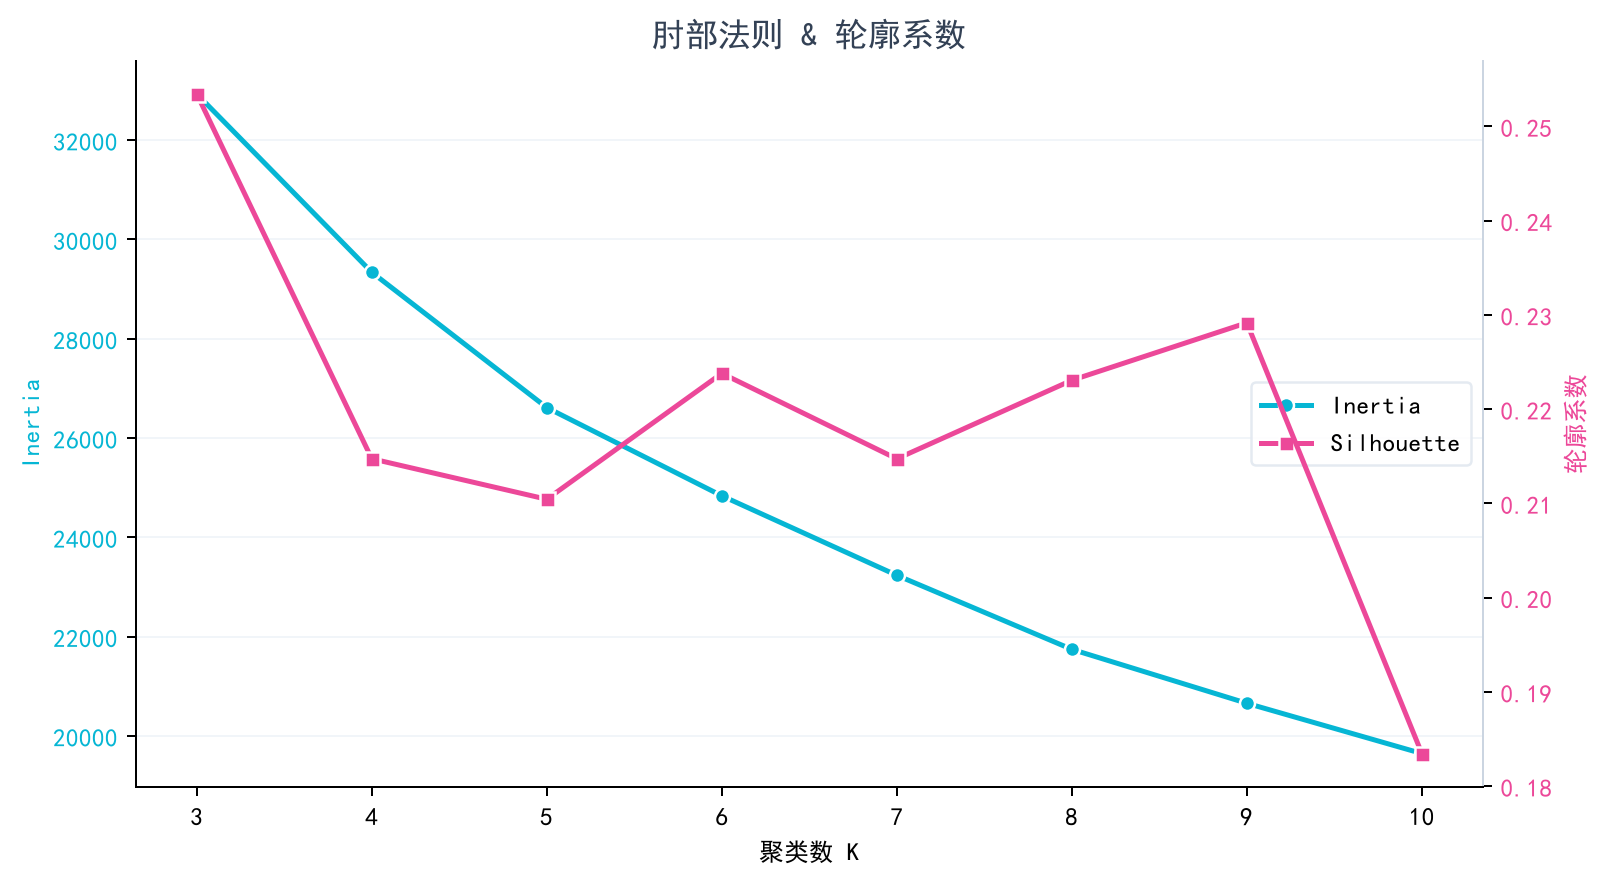
\includegraphics[width=0.88\textwidth]{17_elbow_silhouette.png}
  \caption{K值搜索中的肘部法则与轮廓系数}
  \label{fig:ksearch}
\end{figure}

图\ref{fig:ksearch}同时呈现惯性曲线和轮廓系数。惯性值随 K 增大持续下降，这是 KMeans 聚类中常见的现象，因为类别数增加会自然压缩类内距离。更值得关注的是边际下降幅度和轮廓系数变化。图中 K 从3增加到更高取值后，惯性下降趋于平缓，而轮廓系数未形成持续提升，意味着过多类别会增加解释复杂度，却未明显改善类别分离效果。因此，3类结构在简洁性、可解释性和类间分离度之间形成较合适的平衡。

\section{可视化分析框架}
图表体系按照从总体到局部、从单变量到多变量的顺序组织。第一层关注市场整体状态，使用指数走势、涨跌家数和成交额图观察市场方向、广度和资金活跃度。第二层关注个股横截面分布，使用小提琴图、收益排名图、波动收益散点图和最大回撤分布图呈现收益与风险差异。第三层关注交易行为，使用换手率散点图、涨跌停排名图和价量相关分布图刻画资金交易和价格响应。第四层关注多维画像，使用 PCA 聚类散点图、雷达图和代表股走势把多指标结果转化为可解释的股票类型。

这一框架将探索性图表和解释性图表结合起来。指数走势和成交额图提供总体背景，分布图和散点图揭示结构差异，聚类图和代表股图则把统计结果转化为类型叙事。色彩设计保持相对稳定，不同聚类在多张图中使用一致颜色，收益正负和上涨下跌保持视觉区分。对于股票数量较多的横截面图，散点透明度用于减轻遮挡，排名图只呈现头部和尾部对象，分布图则用整体形态替代逐点展示，从而降低阅读负担。

\section{大盘全景分析}
中证2000在样本期内呈现出先抬升、后回撤、再修复的阶段特征。图\ref{fig:index}中蓝色折线表示指数收盘价，黄绿色折线表示 MA5，深色折线表示 MA20。指数在1月初至2月上旬整体上行，随后进入震荡区间。3月下旬出现明显回撤，短期低点接近样本期底部。4月以后指数逐步修复，并在5月中旬附近达到阶段高位，随后又出现回落。MA5 对短期波动反应较快，MA20 更能反映中期趋势。两条均线在3月回撤和4月修复阶段出现明显分离，反映市场状态经历了短期冲击和趋势修复之间的转换。

\begin{figure}[H]
  \centering
  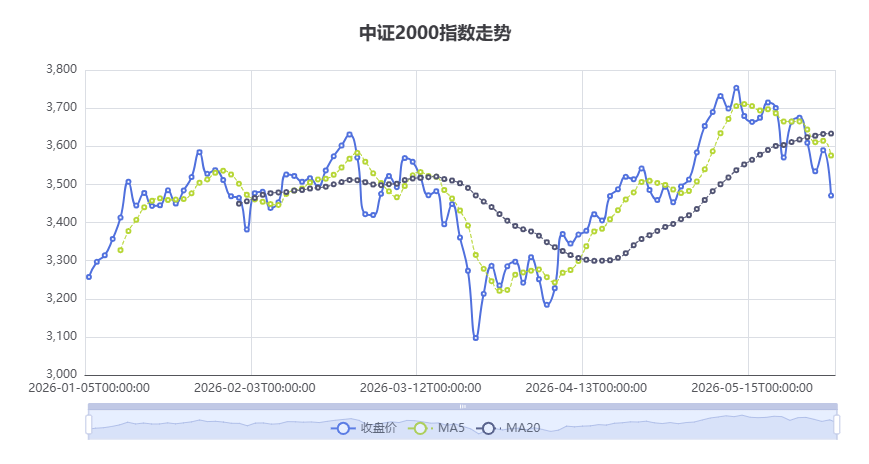
\includegraphics[width=0.95\textwidth]{01_index_line_cropped.png}
  \caption{中证2000指数走势与移动均线}
  \label{fig:index}
\end{figure}

涨跌家数揭示了指数背后的市场广度。图\ref{fig:updown}用红色表示上涨家数、灰色表示平盘家数、绿色表示下跌家数。红绿柱体在不同交易日之间快速切换，表明市场内部情绪变化较快，并非始终沿着单一方向演化。在市场回撤阶段，下跌家数显著增加，市场风险由个股扩散到更宽的股票池。反弹阶段上涨家数增加，表明情绪改善并非完全来自少数股票。由于中证2000成分股权重相对分散，涨跌家数比指数点位更能反映中小市值股票的内部强弱。

\begin{figure}[H]
  \centering
  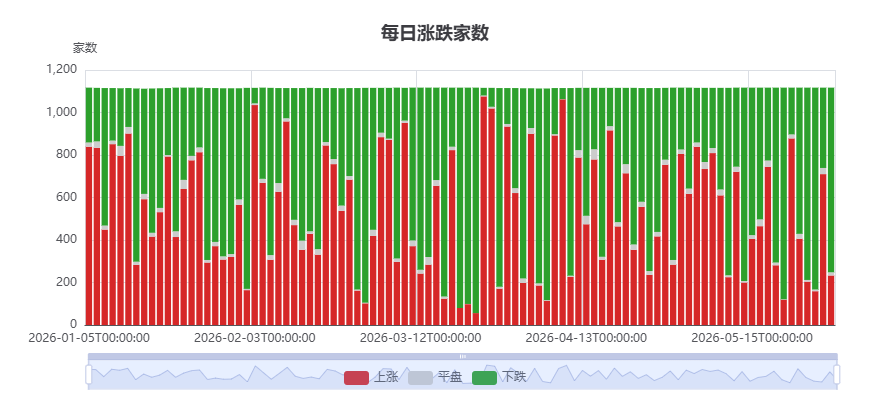
\includegraphics[width=0.95\textwidth]{02_daily_up_down_cropped.png}
  \caption{每日上涨、平盘与下跌家数}
  \label{fig:updown}
\end{figure}

成交额变化补充了资金参与度线索。图\ref{fig:amount}的面积和折线共同显示，样本期成分股日成交额并非平稳序列，而是在若干阶段出现放量。1月和5月附近的成交额高点对应更活跃的资金交换，3月至4月的量能收缩则与市场回撤和修复之间的犹豫状态相呼应。结合指数走势观察，放量上涨通常意味着资金参与度提高，放量下跌则提示风险释放和换手加剧。成交额本身不直接给出收益结论，却能为量价关系、聚类画像和典型个股分析提供市场背景。

\begin{figure}[H]
  \centering
  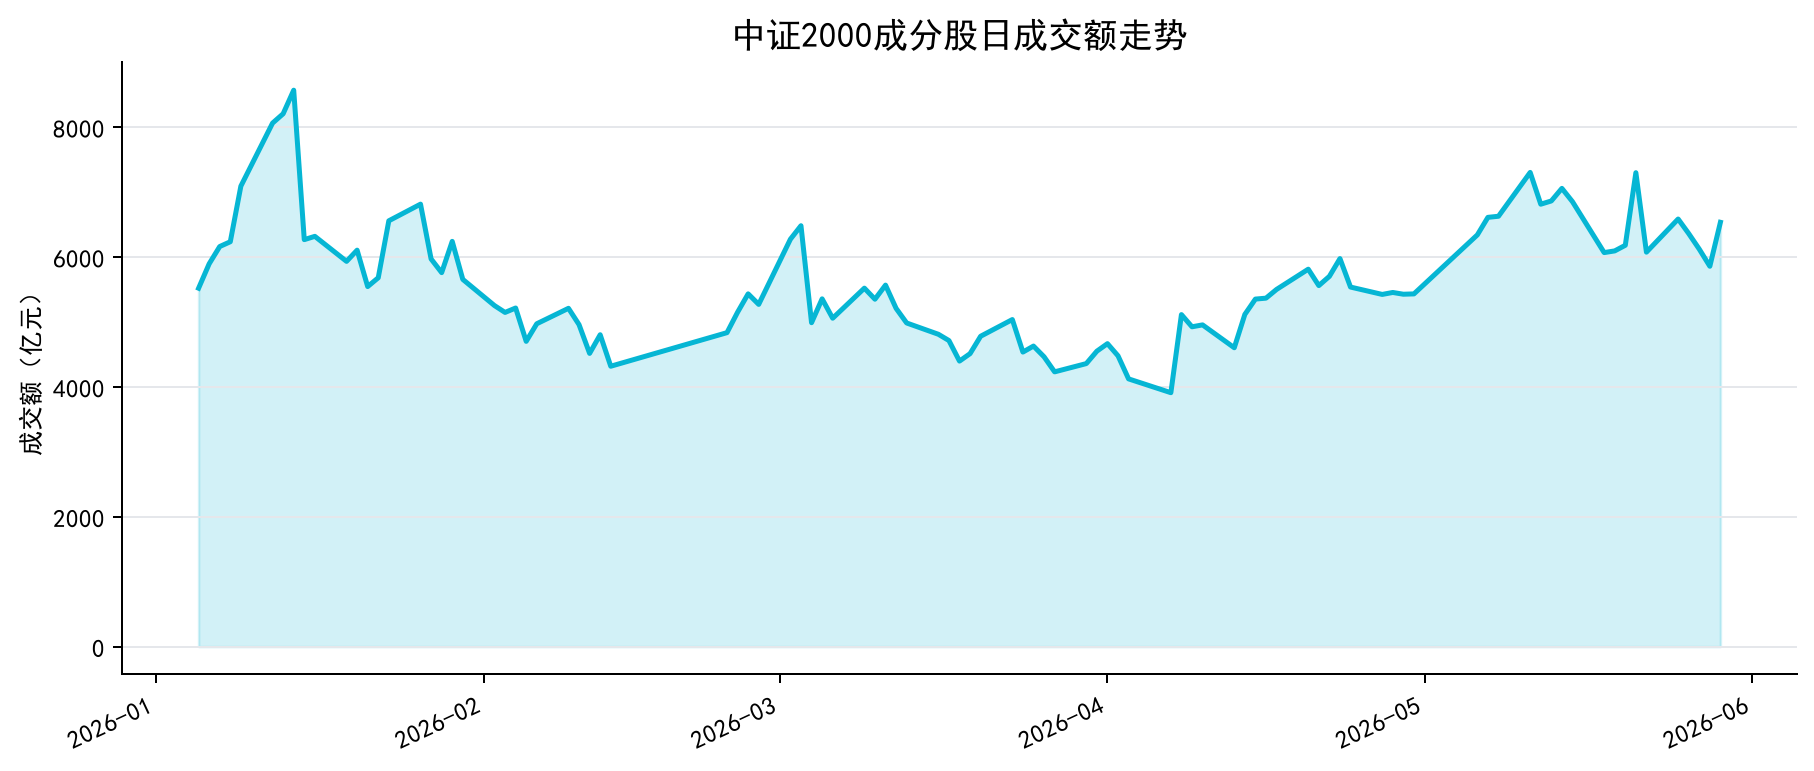
\includegraphics[width=0.88\textwidth]{05_daily_amount.png}
  \caption{成分股日成交额走势}
  \label{fig:amount}
\end{figure}

\section{风险收益结构}
月度收益分布显示，指数变化不能替代个股层面的实际表现。图\ref{fig:violin}中的小提琴宽度代表该收益区间内股票数量的集中程度，中位数和分布尾部则反映当月收益的中心位置与极端表现。部分月份分布较宽，表明个股表现分化强烈；部分月份中位数偏低，提示多数股票承压。该图把时间分组与横截面分布结合起来，使市场阶段和个股离散程度能够同时被观察。由此可以理解，指数层面的阶段性修复并不必然意味着个股收益分布整体上移，分布形态本身才是判断市场质量的重要证据。

\begin{figure}[H]
  \centering
  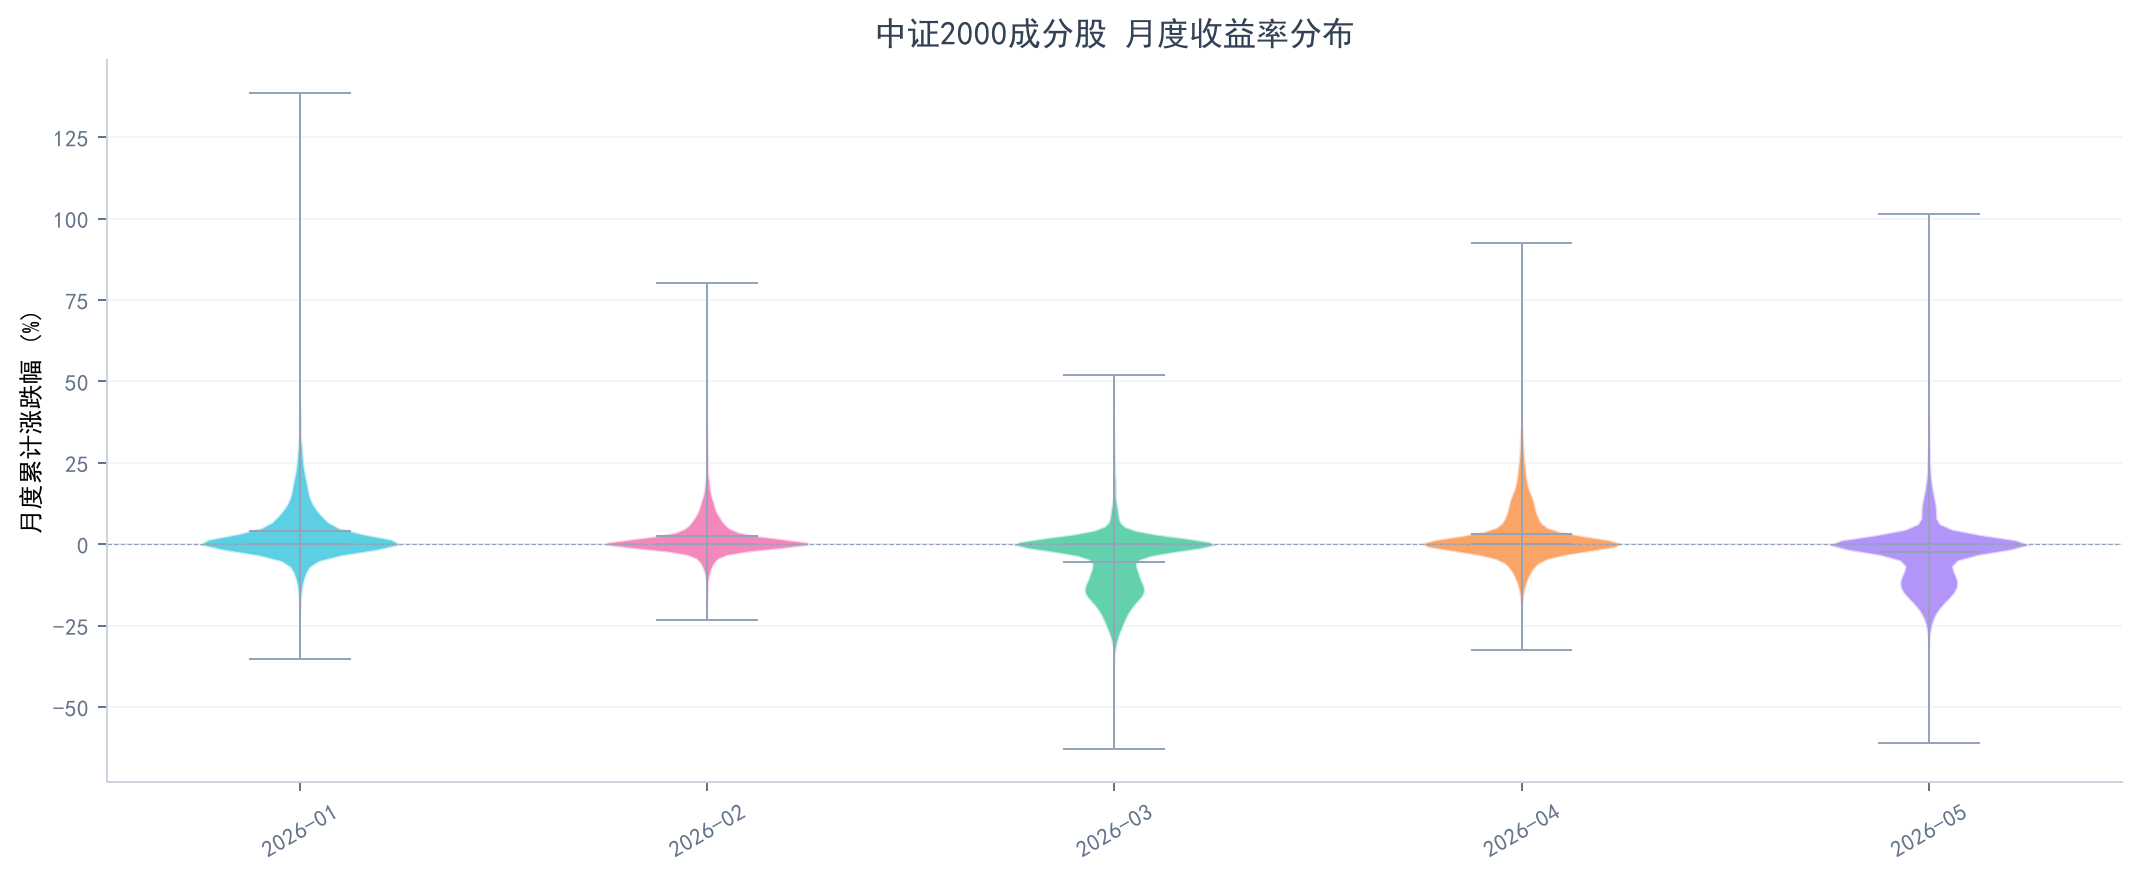
\includegraphics[width=0.88\textwidth]{03_monthly_return_violin.png}
  \caption{月度收益率横截面分布}
  \label{fig:violin}
\end{figure}

累计收益排名进一步放大了头尾分化。图\ref{fig:topbottom}将收益率最高和最低的股票放在同一视图中，条形长度直接反映个股在样本期内的累计涨跌幅。头部股票贡献显著正收益，尾部股票则出现较大跌幅，二者之间的距离远大于指数层面的波动幅度。该图表明中证2000内部并不是均质资产池，主题轮动、流动性变化和个股事件会共同放大分化。若分析只观察指数，容易忽视股票池内部同时存在的强势股和弱势股。

\begin{figure}[H]
  \centering
  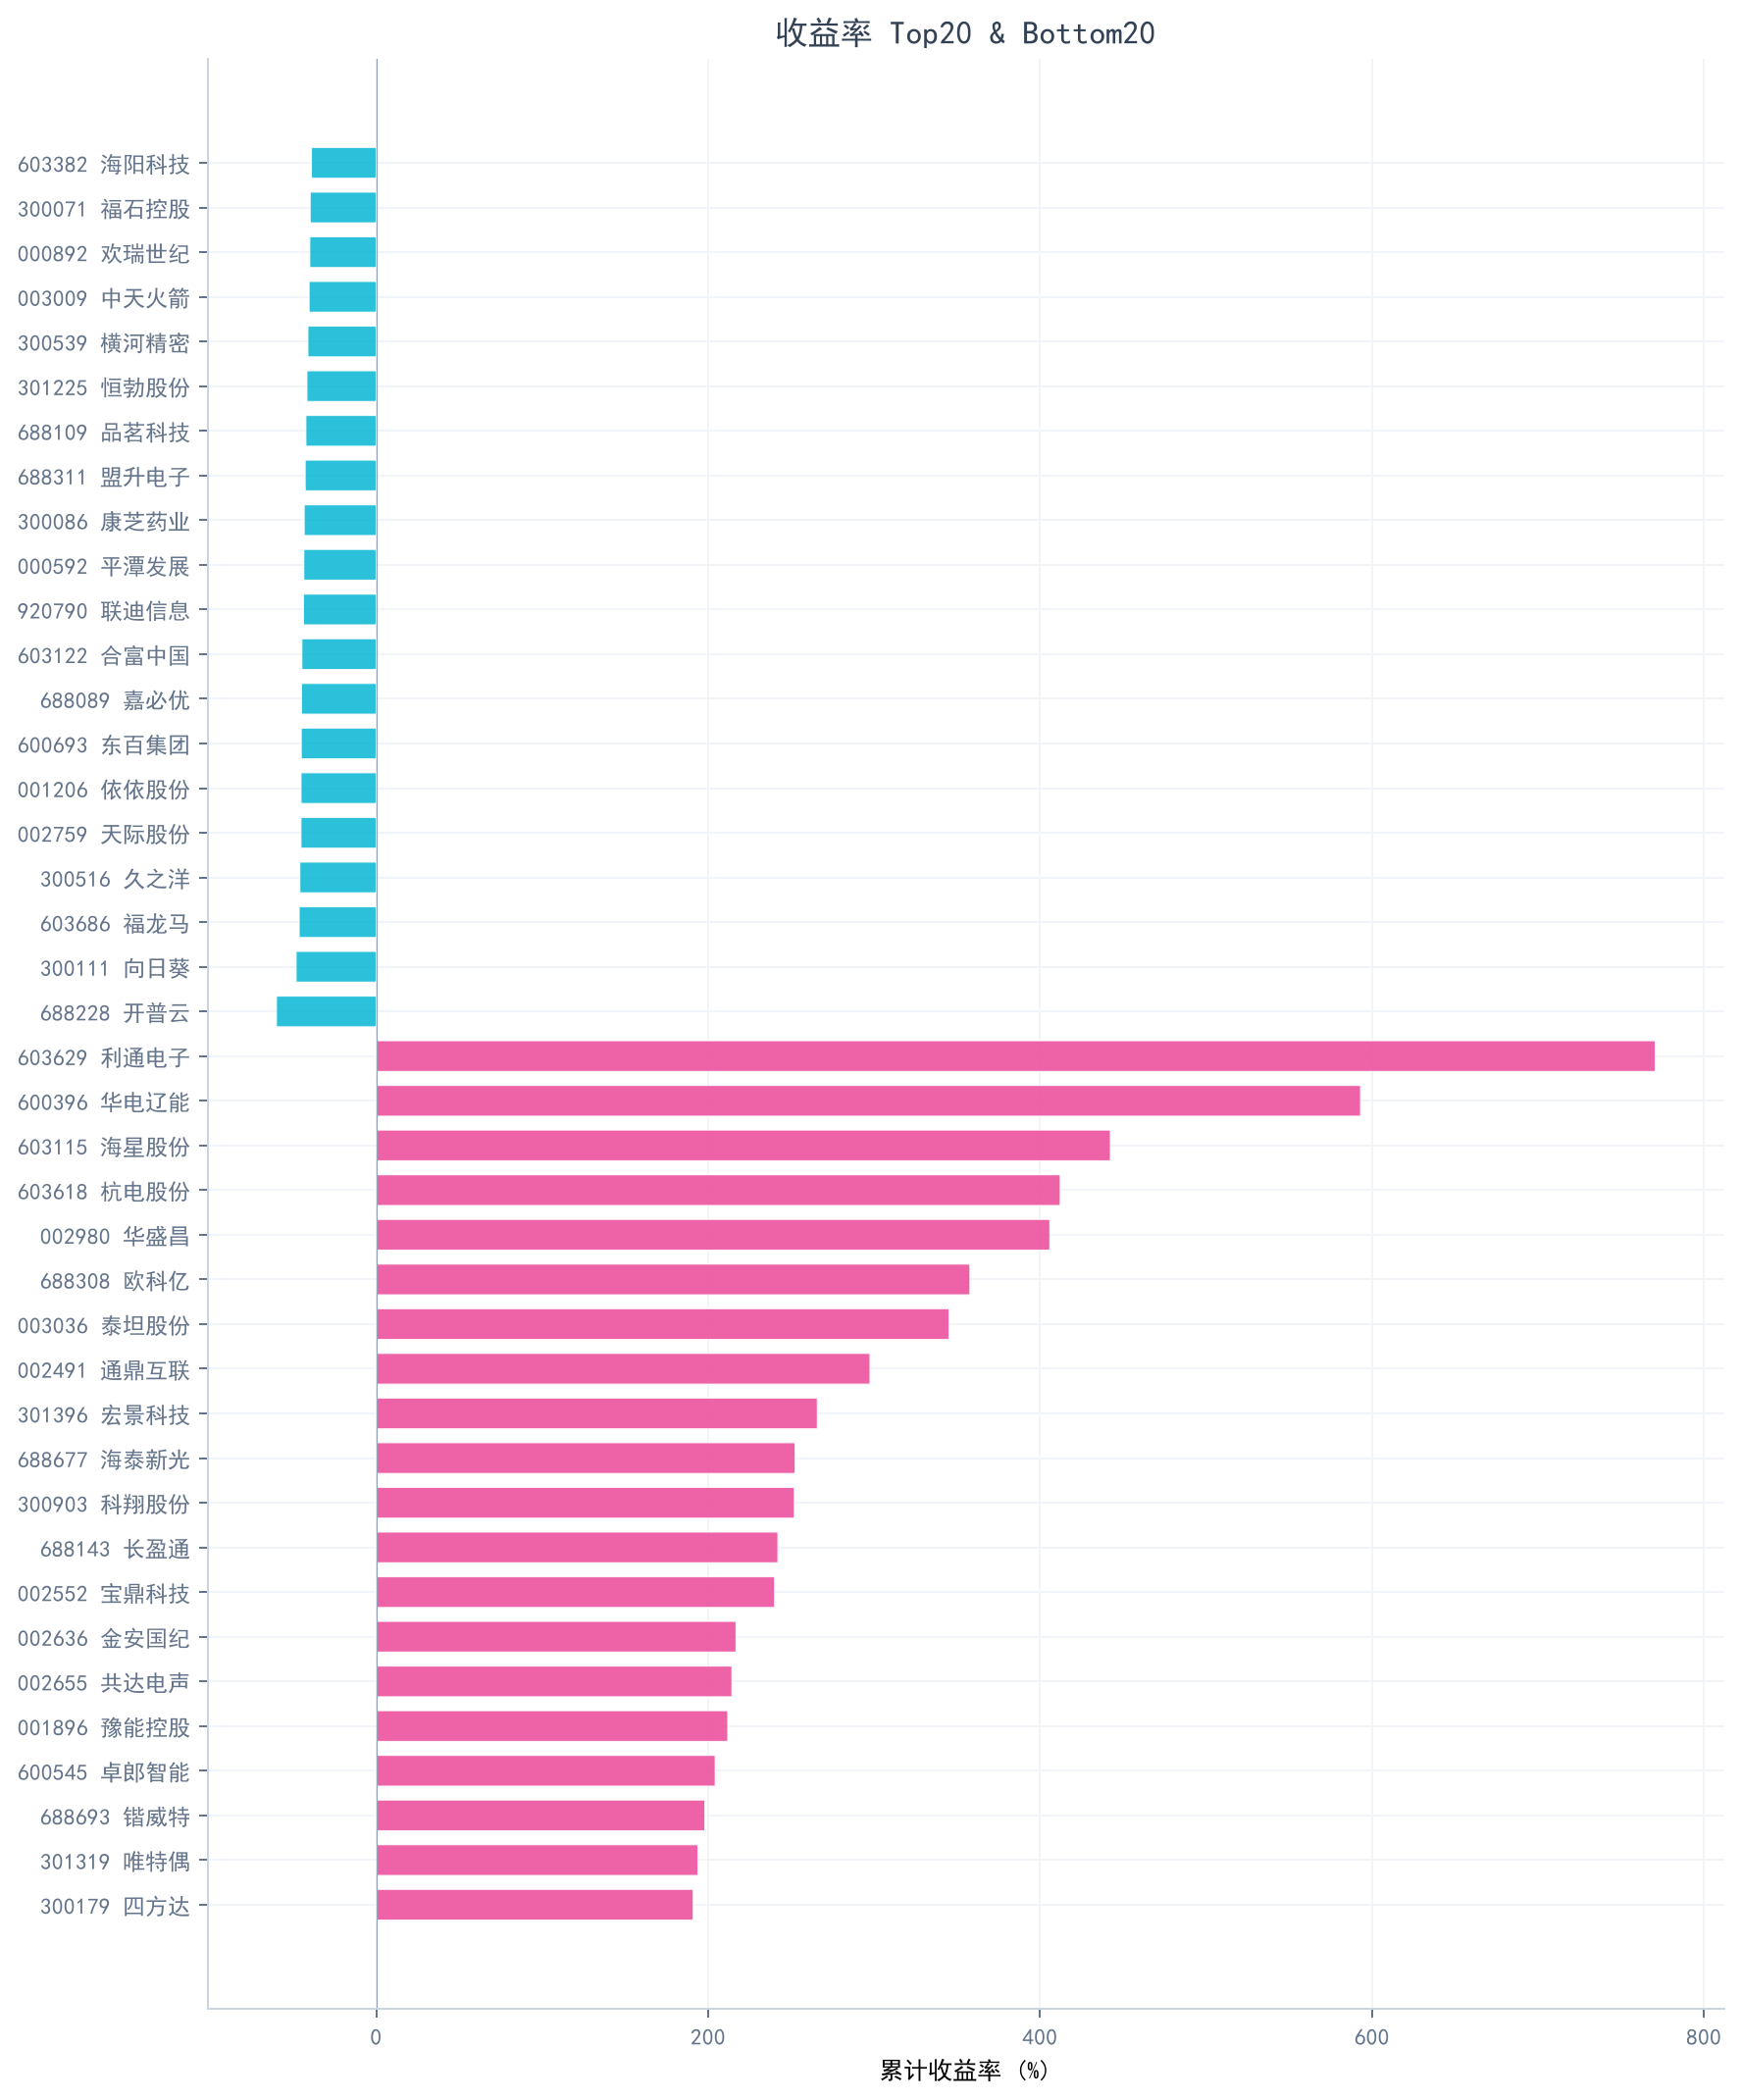
\includegraphics[width=0.82\textwidth]{04_top_bottom_returns.png}
  \caption{累计收益率前20与后20股票}
  \label{fig:topbottom}
\end{figure}

波动率与收益率的关系揭示了不同收益来源的差异。图\ref{fig:volret}中，每个点代表一只股票，横轴为年化波动率，纵轴为累计收益率，颜色表示聚类类型。点云的分散程度表明高收益股票并不集中在单一风险区间。放量突破型股票整体收益较高，但并非全部处于最高波动区域，表明其收益优势不只来自风险暴露。高弹性反弹型股票波动率和换手率更高，收益分布也更分散。低流动性型股票数量最多，平均收益偏弱，提示低活跃度并不天然带来防御属性。

\begin{figure}[H]
  \centering
  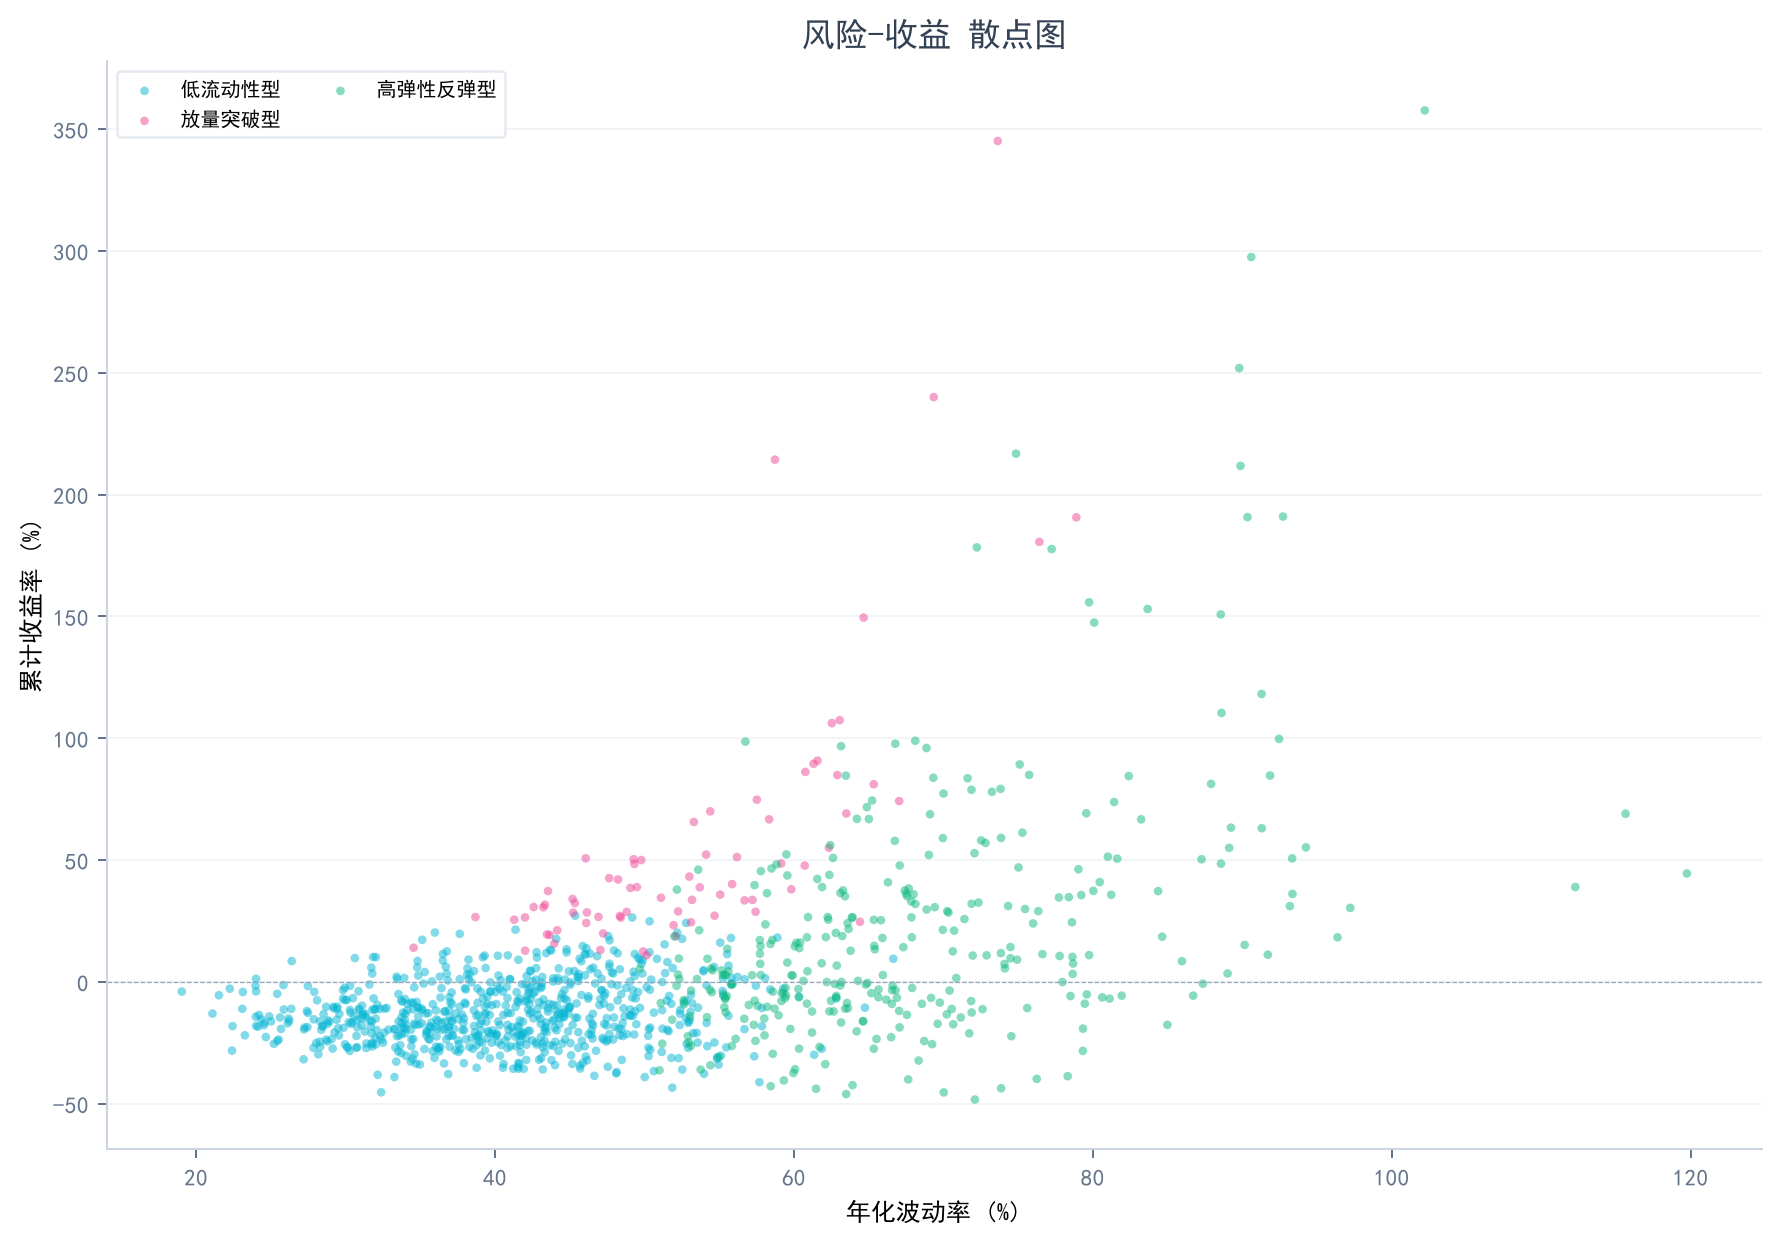
\includegraphics[width=0.88\textwidth]{06_volatility_vs_return.png}
  \caption{年化波动率与累计收益率关系}
  \label{fig:volret}
\end{figure}

最大回撤分布刻画了持有过程中的下行风险。图\ref{fig:drawdown}中柱形越高，表示落在对应回撤区间的股票越多；左尾越长，表示深度回撤样本越多。成分股最大回撤集中在负值区间，且左尾较长。即使样本期指数在4月以后修复，许多个股仍经历较深回撤。最大回撤需要与累计收益同时观察。收益高且回撤相对可控的股票更可能代表稳定强势；收益高但回撤极深的股票则更多体现高弹性和高不确定性。

\begin{figure}[H]
  \centering
  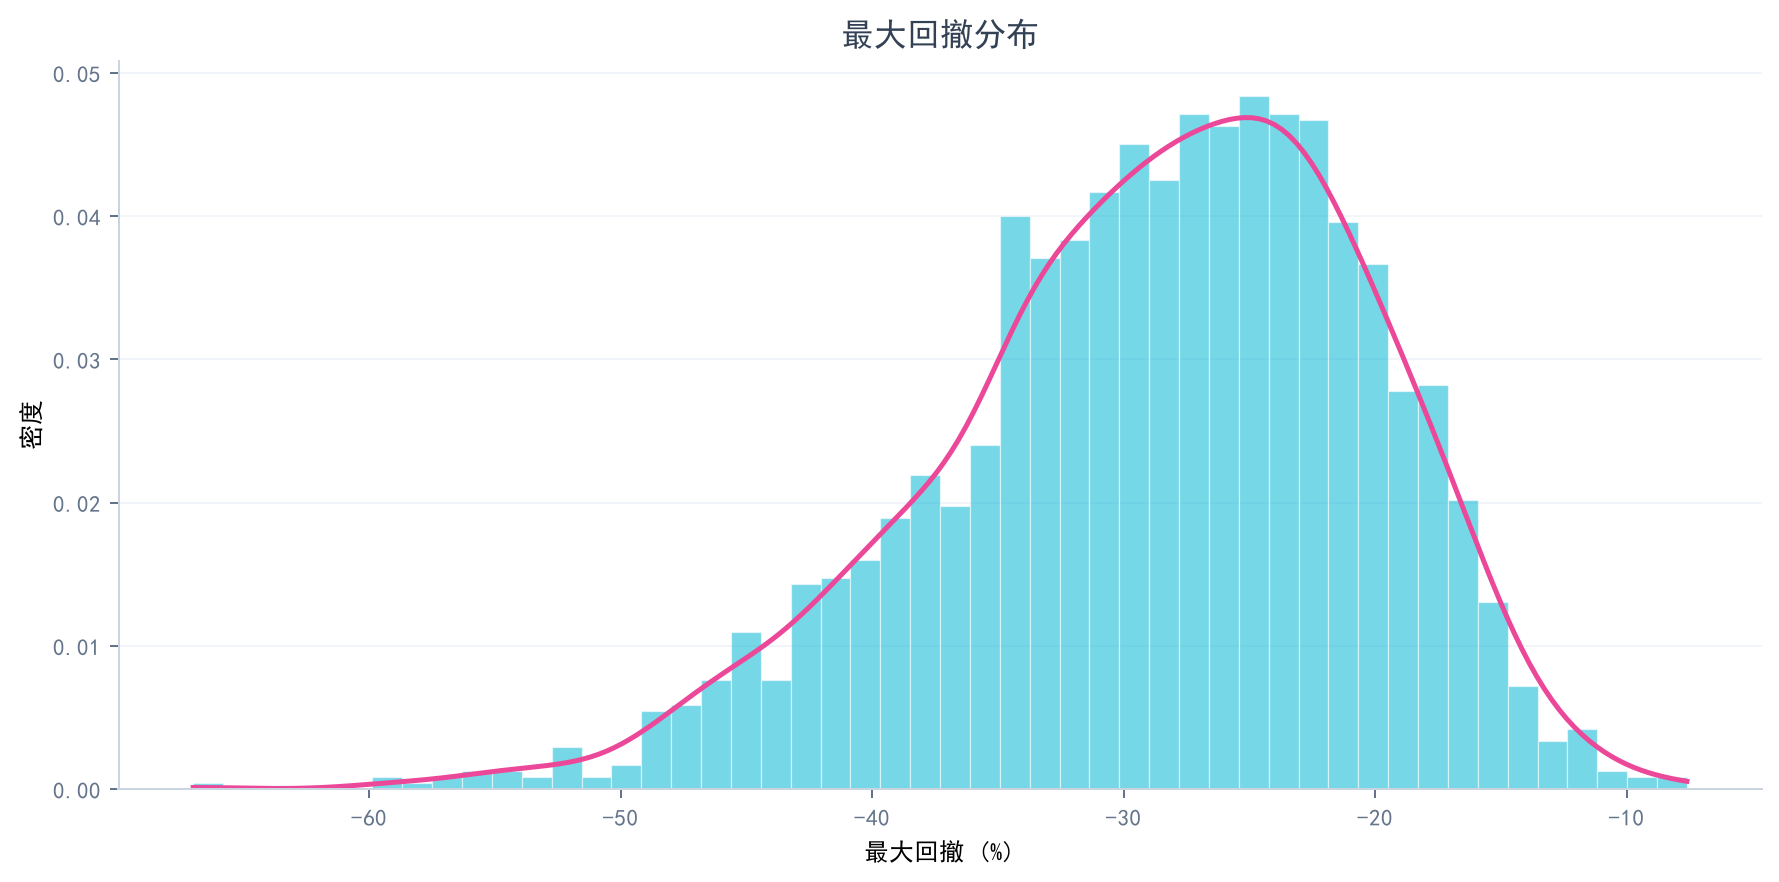
\includegraphics[width=0.88\textwidth]{07_max_drawdown_hist.png}
  \caption{最大回撤分布}
  \label{fig:drawdown}
\end{figure}

\section{量价异动与交易行为}
交易活跃度是理解中小市值股票分化的重要线索。图\ref{fig:turnover}以平均换手率为横轴、累计收益率为纵轴，展示交易活跃度与价格表现之间的关系。点云并未沿着单调上升方向排列，表明高换手股票并不必然获得更高收益。高弹性反弹型股票明显集中在换手率较高区域，表明资金交易活跃度与价格弹性之间存在联系。低流动性型股票换手率较低，收益均值也偏弱，反映出流动性不足可能限制价格修复速度。放量突破型股票虽然平均换手率不高，但收益均值最高，其关键并非持续高换手，而可能是阶段性放量与趋势突破的组合。

\begin{figure}[H]
  \centering
  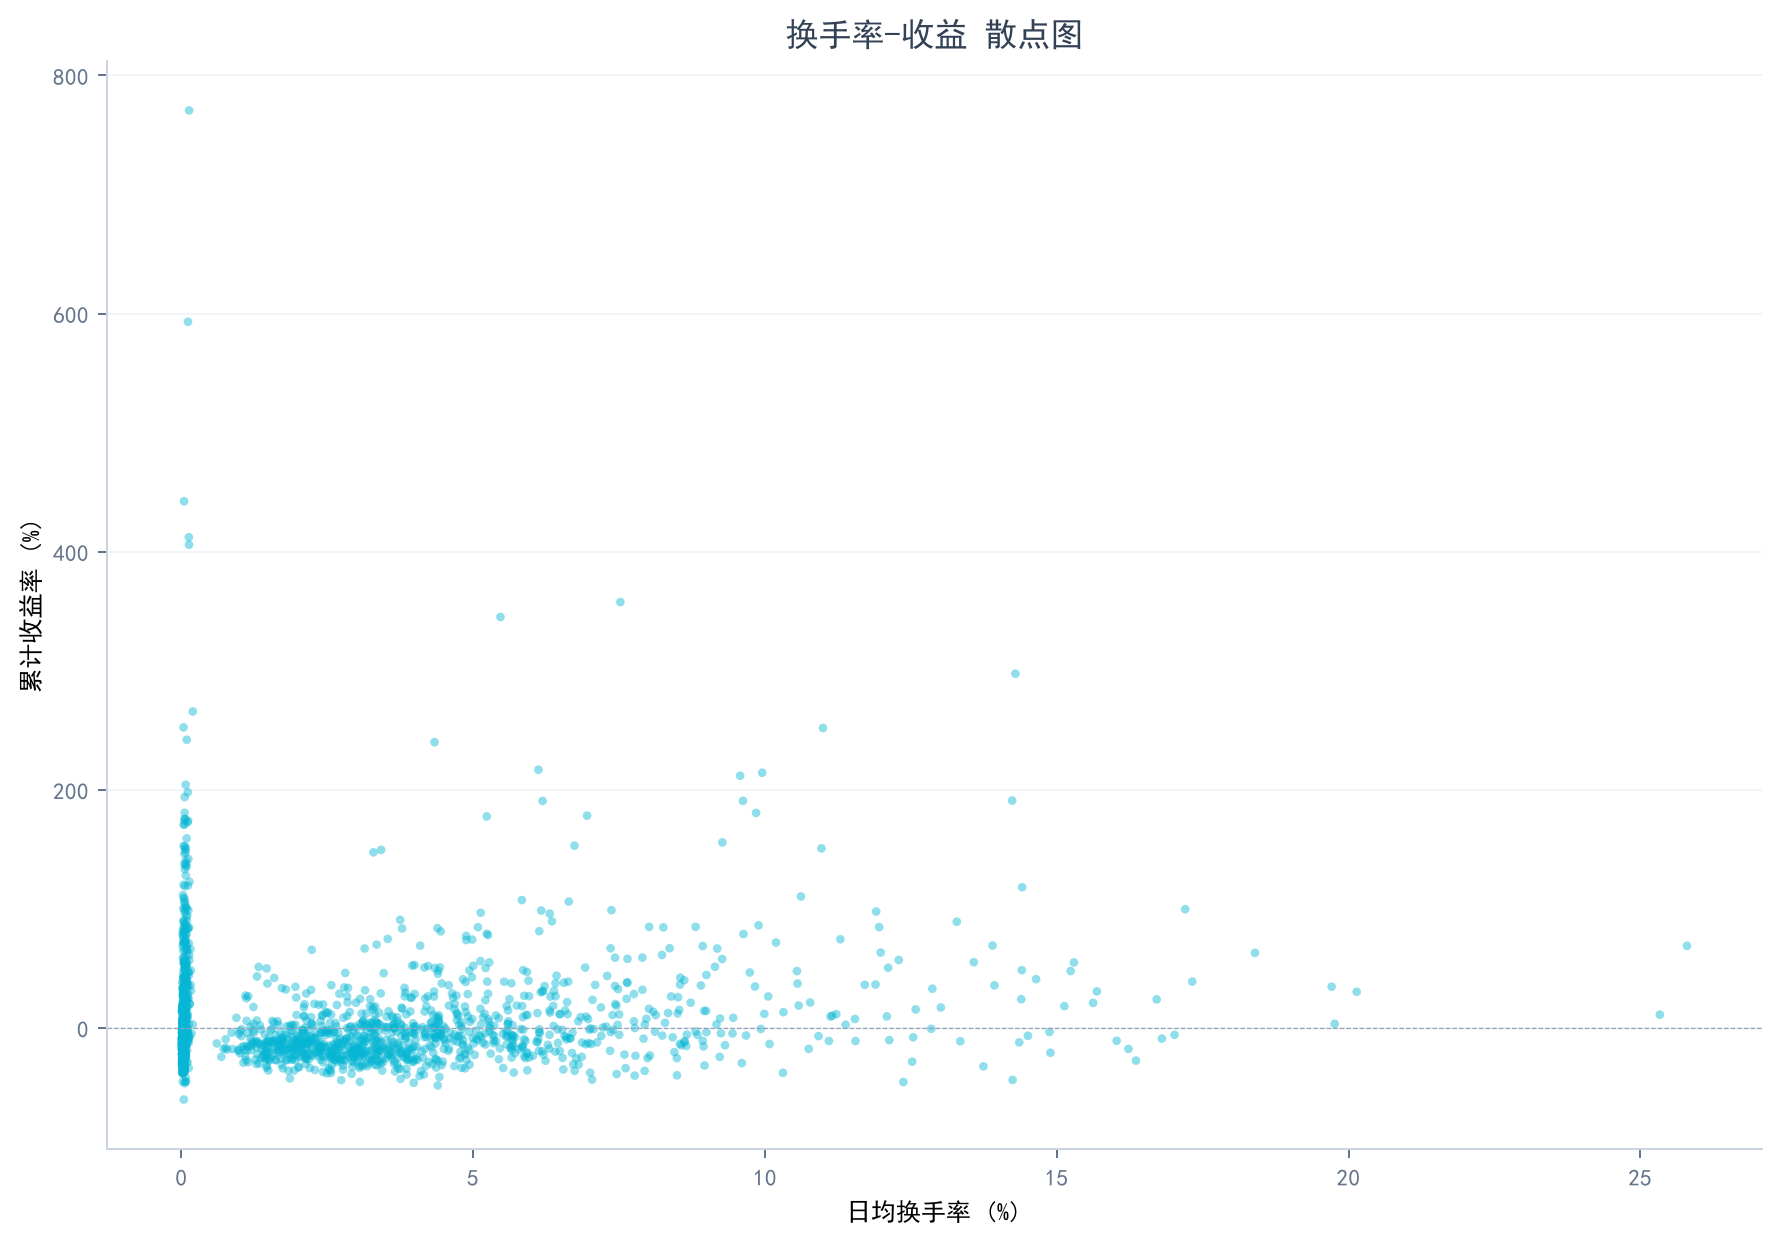
\includegraphics[width=0.88\textwidth]{10_turnover_vs_return.png}
  \caption{平均换手率与累计收益率关系}
  \label{fig:turnover}
\end{figure}

涨停和跌停次数体现了极端交易行为的集中程度。图\ref{fig:limit}通过排名方式突出极端事件较多的股票，避免大量普通样本稀释异常信息。部分股票在样本期内多次触及涨停或跌停，显示中证2000内部存在较强的事件驱动和短期情绪波动。涨停次数较多的股票可能对应资金追逐和主题强化，跌停次数较多的股票则可能存在流动性冲击或基本面压力。该图不直接形成投资判断，而是帮助识别需要进一步解释的异常对象。

\begin{figure}[H]
  \centering
  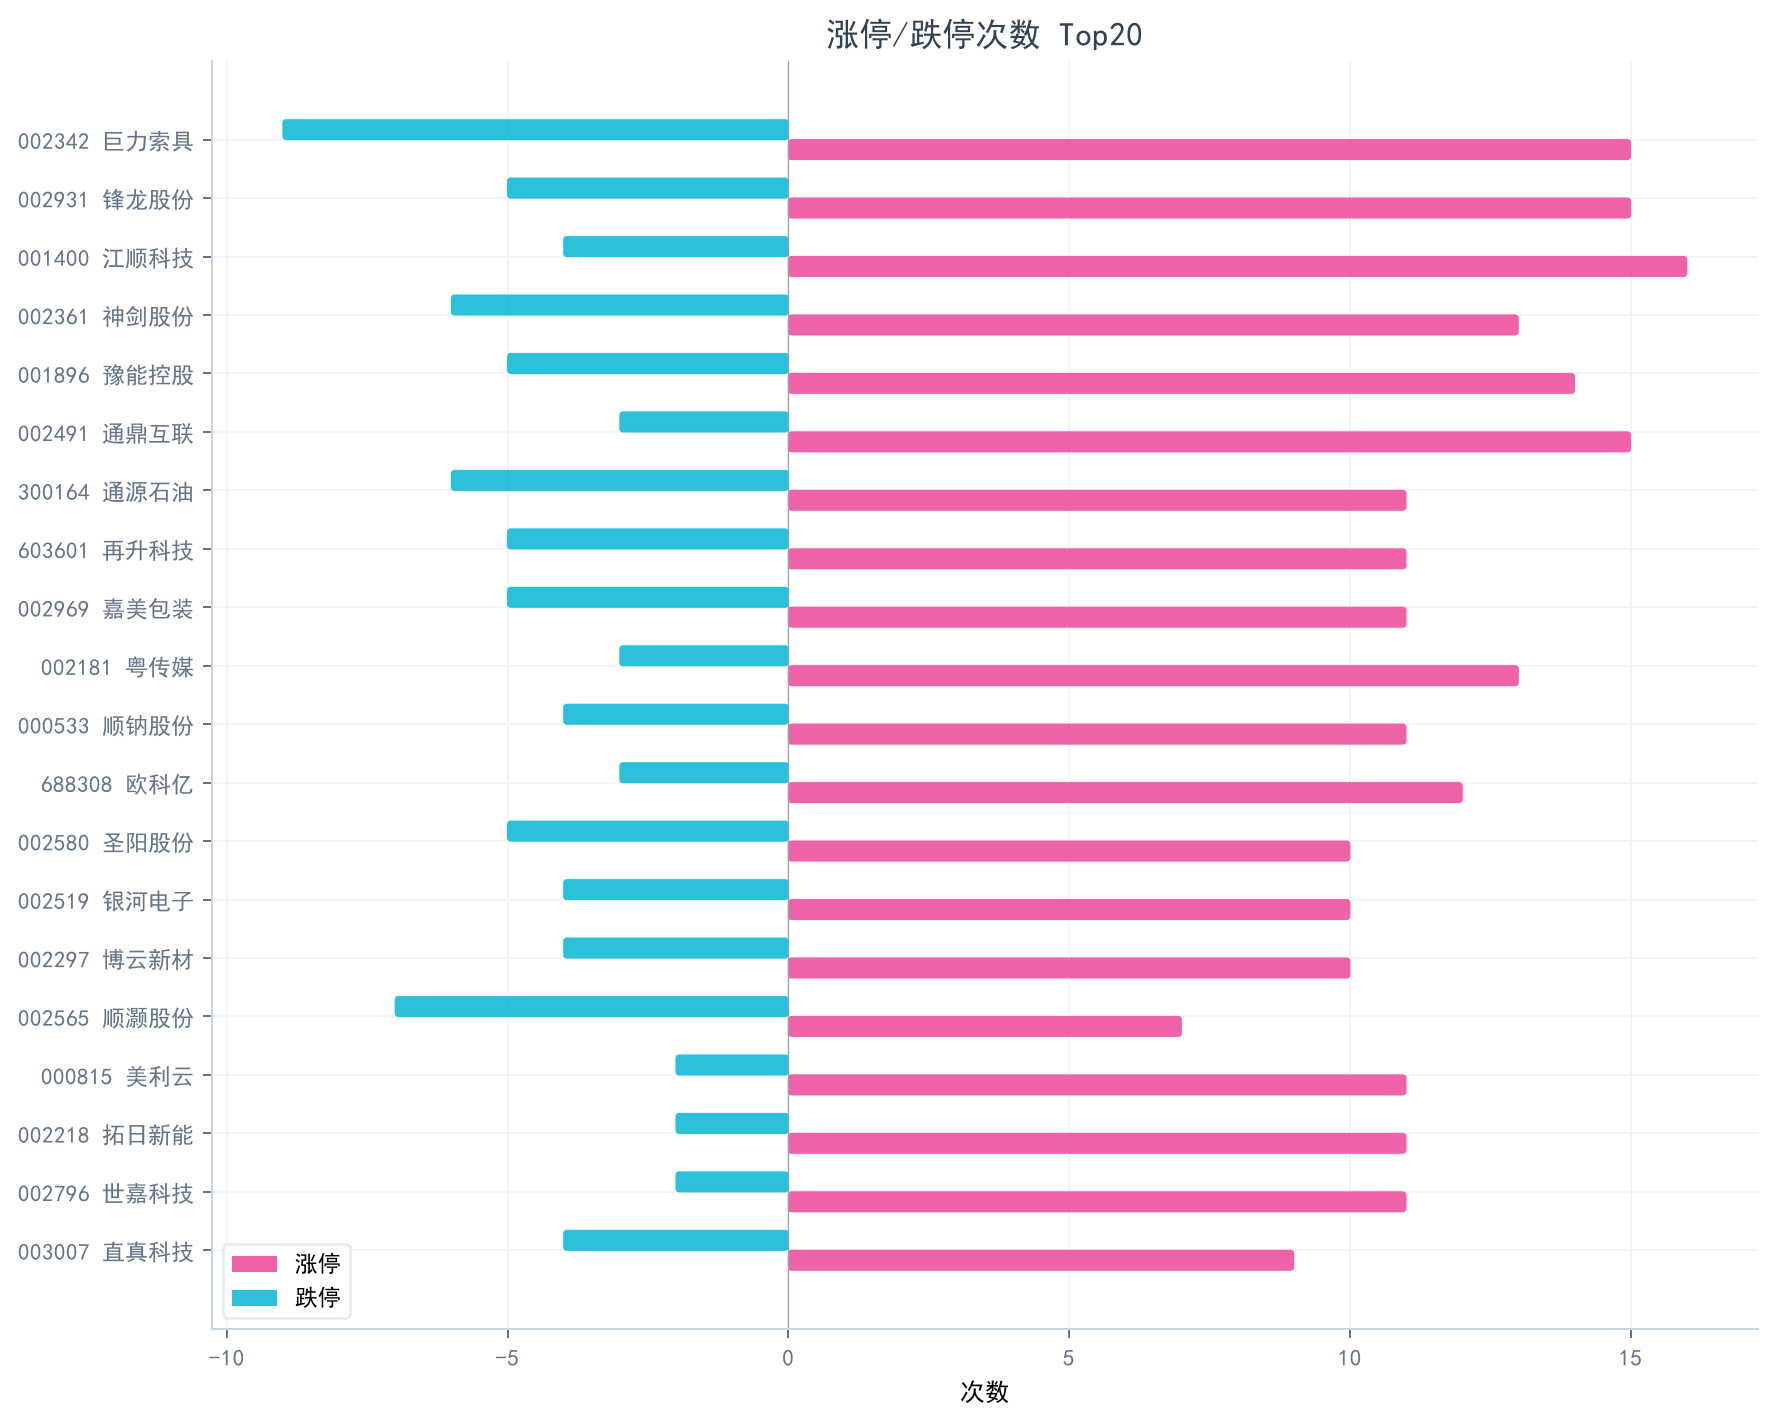
\includegraphics[width=0.88\textwidth]{11_limit_up_down_top.png}
  \caption{涨停和跌停次数排名}
  \label{fig:limit}
\end{figure}

价量相关系数刻画价格变化与成交量变化的同步程度。图\ref{fig:pvcorr}的分布主体集中在中间区域，显示多数股票的价量相关关系并不极端，表明单一量价同步指标不足以解释所有股票表现。右侧正相关区域可能意味着上涨伴随放量，左侧负相关区域可能意味着下跌放量或反弹缩量。将该指标纳入聚类特征，而不单独作为判断标准，更符合多变量共同作用的市场特征。

\begin{figure}[H]
  \centering
  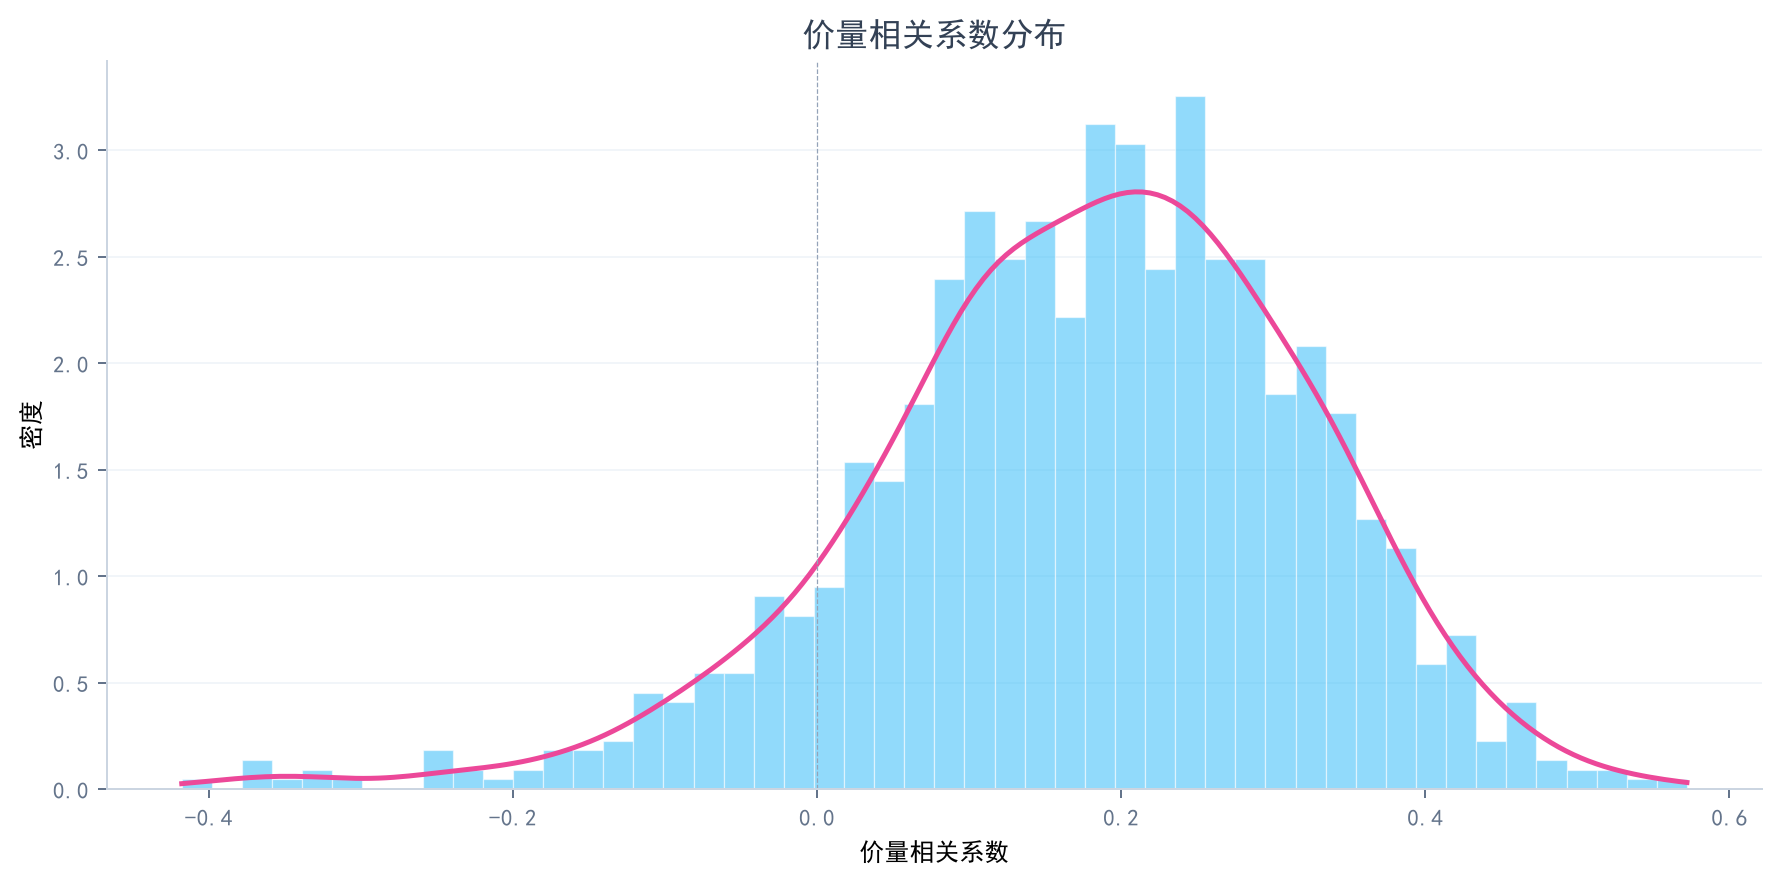
\includegraphics[width=0.88\textwidth]{15_price_volume_corr_hist.png}
  \caption{价量相关系数分布}
  \label{fig:pvcorr}
\end{figure}

\section{聚类画像分析}
PCA 聚类散点图把29个标准化特征压缩到二维空间，使股票类型之间的边界更易观察。图\ref{fig:pca}中每个点代表一只股票，颜色表示聚类类别，横纵轴分别对应前两个主成分方向。低流动性型股票数量最多，在二维空间中形成较密集的主体区域。放量突破型股票与高弹性反弹型股票分布更分散，表明它们在收益、波动、换手和形态指标上与主体样本存在明显差异。二维图不能替代全部高维信息，但能帮助读者直观理解聚类结果并非随机标签，而是由特征结构支撑的分组。

\begin{figure}[H]
  \centering
  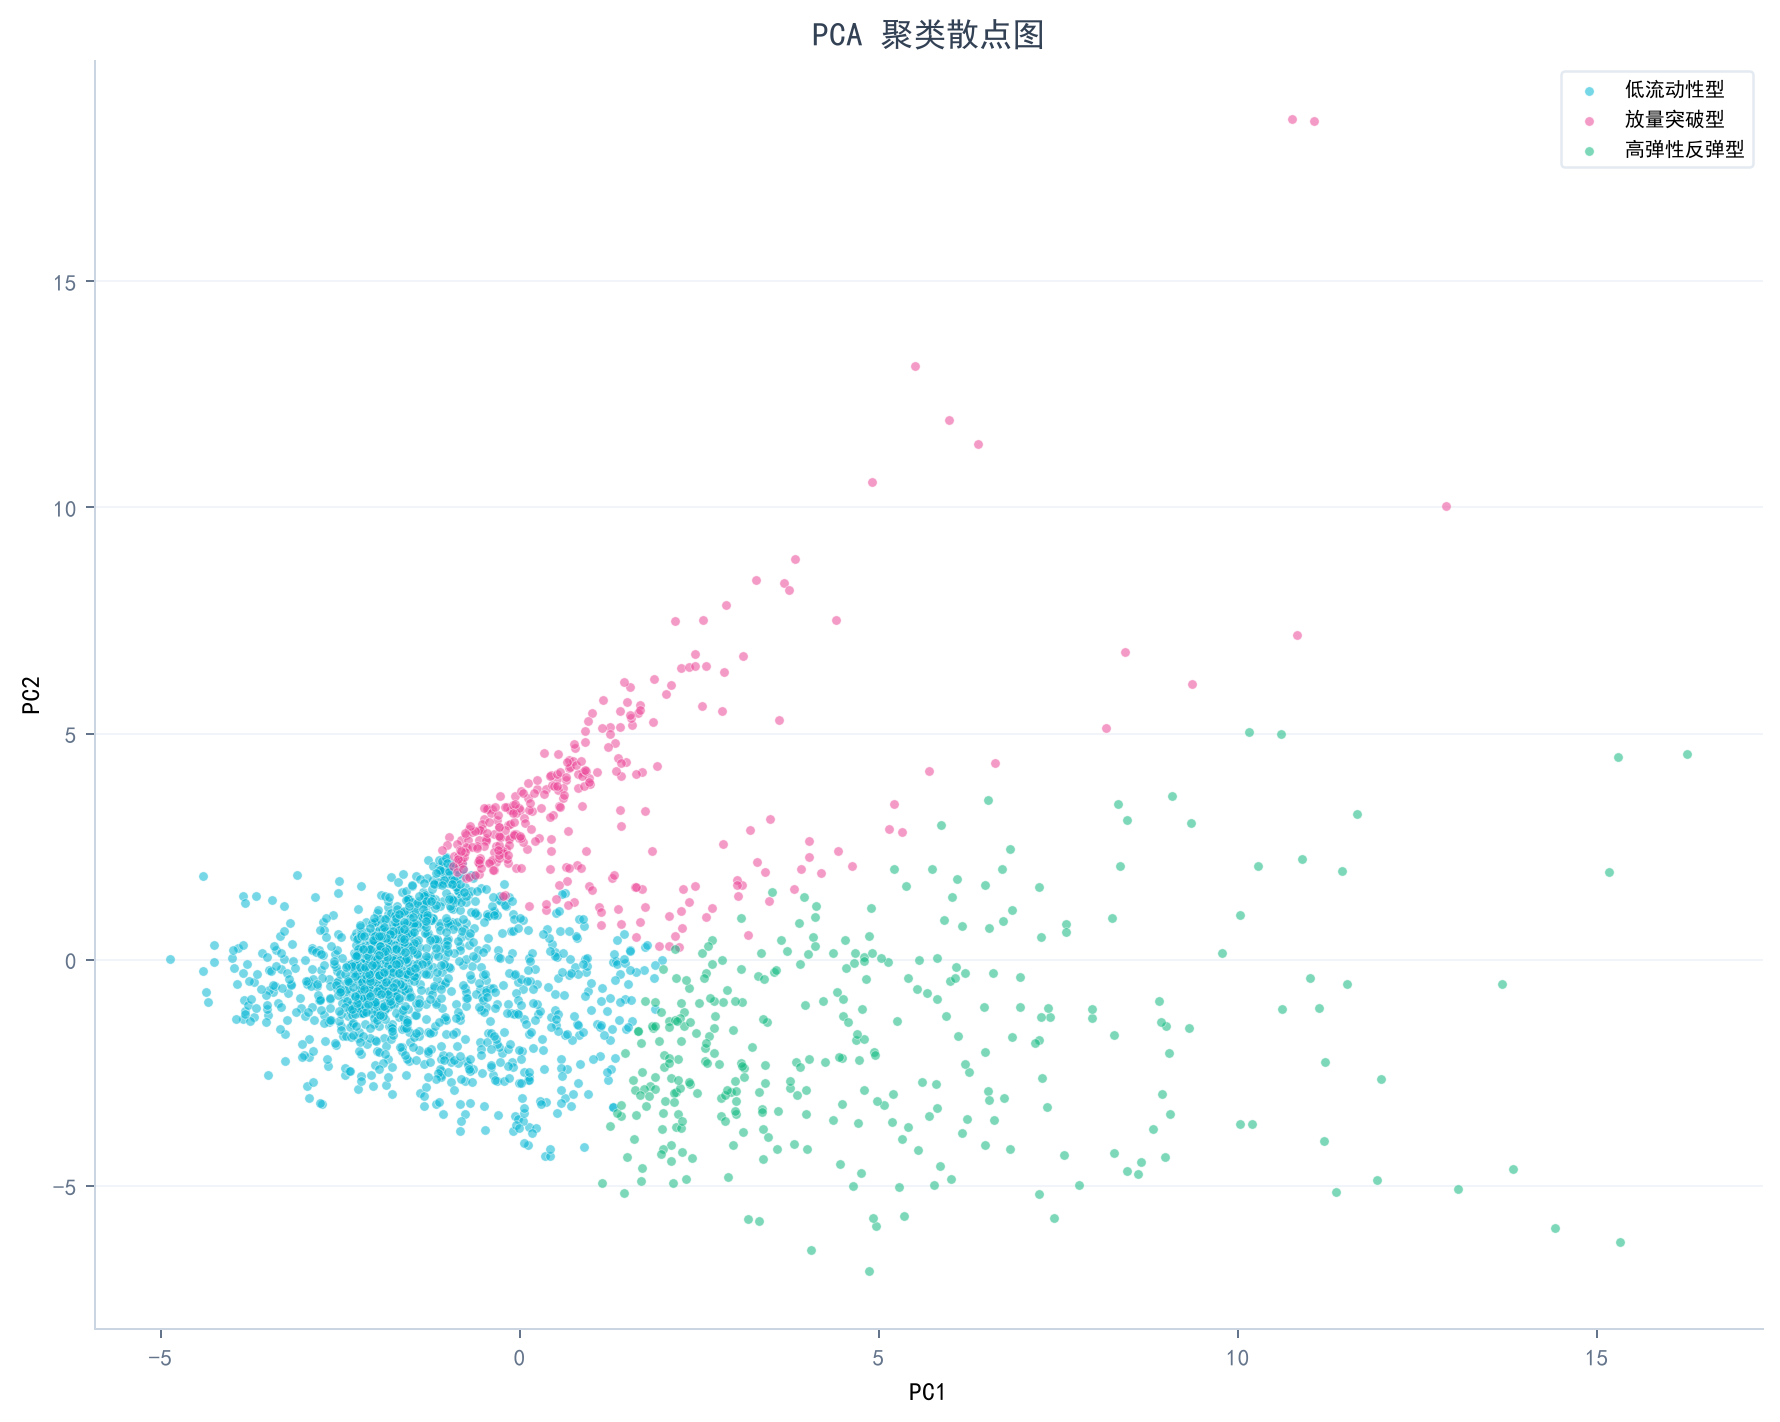
\includegraphics[width=0.88\textwidth]{16_pca_cluster_scatter.png}
  \caption{PCA 二维聚类散点图}
  \label{fig:pca}
\end{figure}

聚类统计表明三类股票具有清晰的风险收益差异。低流动性型包含1,362只股票，是样本中的主导类别，平均收益率为 -12.502，平均波动率为40.543，平均最大回撤为 -28.619，平均换手率为1.708。放量突破型包含312只股票，平均收益率达到67.919，平均最大回撤为 -24.063，平均换手率为1.094。高弹性反弹型包含326只股票，平均收益率为21.429，平均波动率为68.201，平均最大回撤为 -33.705，平均换手率为7.789。

\begin{table}[H]
  \centering
  \caption{三类股票画像统计}
  \label{tab:cluster}
  \begin{tabular}{lrrrrrr}
    \toprule
    类型 & 数量 & 平均收益 & 平均波动 & 平均回撤 & 平均换手 & 平均振幅 \\
    \midrule
    放量突破型 & 312 & 67.919 & 53.214 & -24.063 & 1.094 & 4.597 \\
    低流动性型 & 1362 & -12.502 & 40.543 & -28.619 & 1.708 & 3.422 \\
    高弹性反弹型 & 326 & 21.429 & 68.201 & -33.705 & 7.789 & 5.530 \\
    \bottomrule
  \end{tabular}
\end{table}

雷达图进一步强化了三类股票的相对画像。图\ref{fig:radar}把收益、波动、回撤、换手、振幅和上涨天数压缩到同一极坐标框架中，折线越靠外表示该类别在对应维度上的相对水平越高。放量突破型在收益维度上最突出，回撤压力相对较小。高弹性反弹型在波动、换手和振幅上明显更高，表明其价格对资金和情绪变化更敏感。低流动性型在多数维度上处于低位或中位，虽然波动较低，但收益表现也较弱。分类结果使可视化分析从单张图扩展为画像解释，能够同时呈现宏观趋势和微观结构。

\begin{figure}[H]
  \centering
  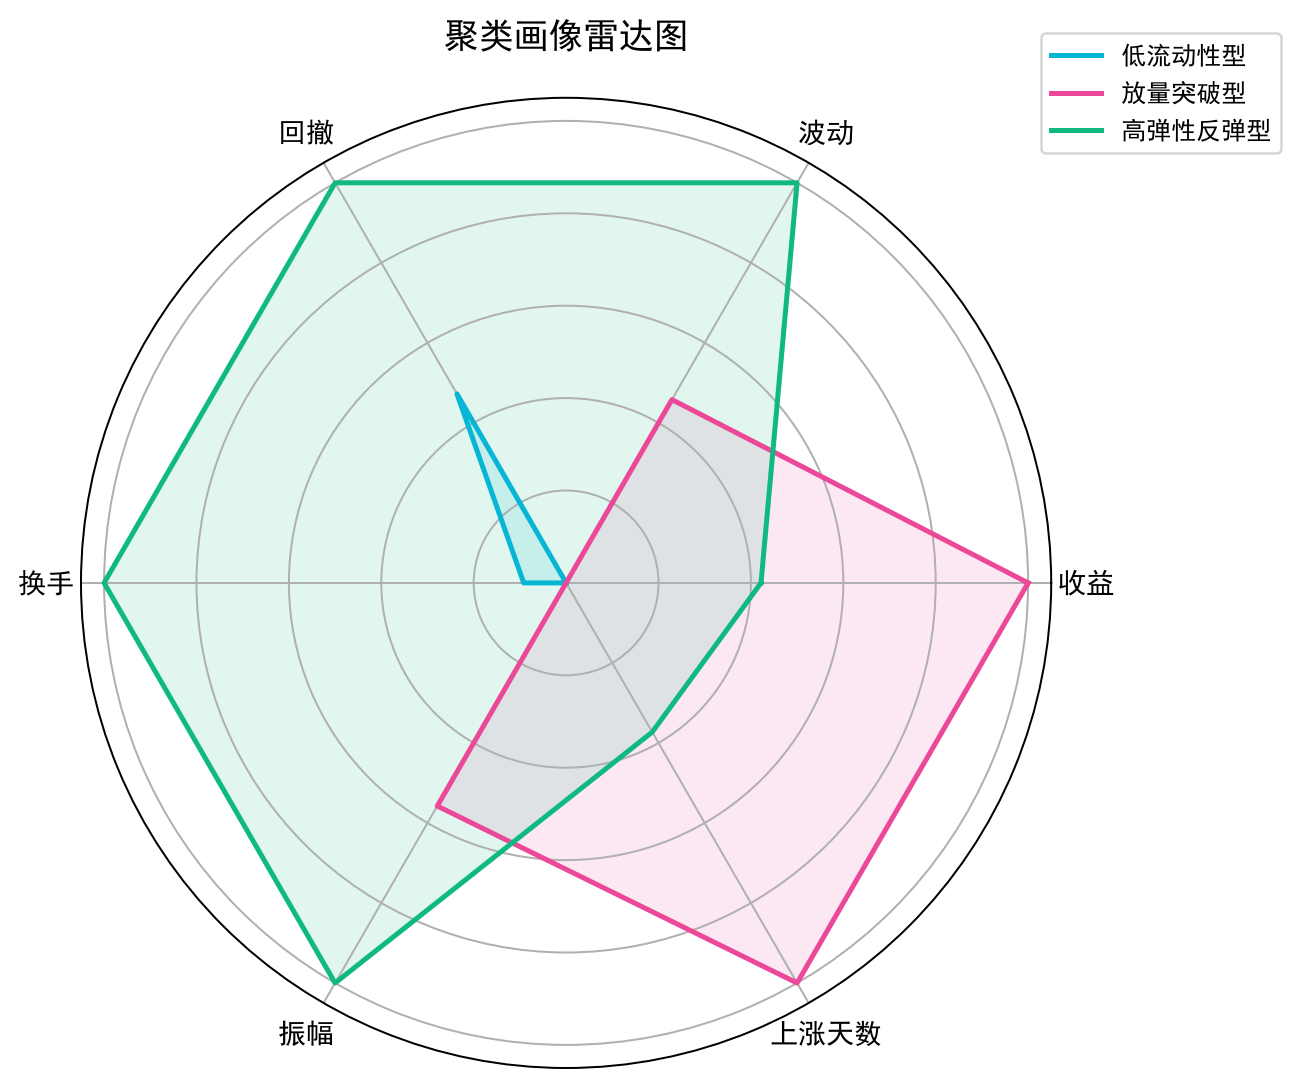
\includegraphics[width=0.78\textwidth]{12_cluster_radar.png}
  \caption{三类股票的相对画像雷达图}
  \label{fig:radar}
\end{figure}

\section{典型个股展示}
代表股走势把聚类画像转化为可观察的时间序列。每一类选取接近该类平均收益的股票作为代表，包括低流动性型中的重庆建工、放量突破型中的新益昌、高弹性反弹型中的昊志机电。图\ref{fig:reprline}将三只代表股的收盘价走势进行归一化对比，起点统一后，曲线间距离可以直接反映相对收益差异。放量突破型代表股在4月以后明显上行，高弹性反弹型代表股波动幅度较大，低流动性型代表股走势更弱。这一对比表明聚类标签并非抽象分类，而能在具体价格轨迹中找到对应形态。

\begin{figure}[H]
  \centering
  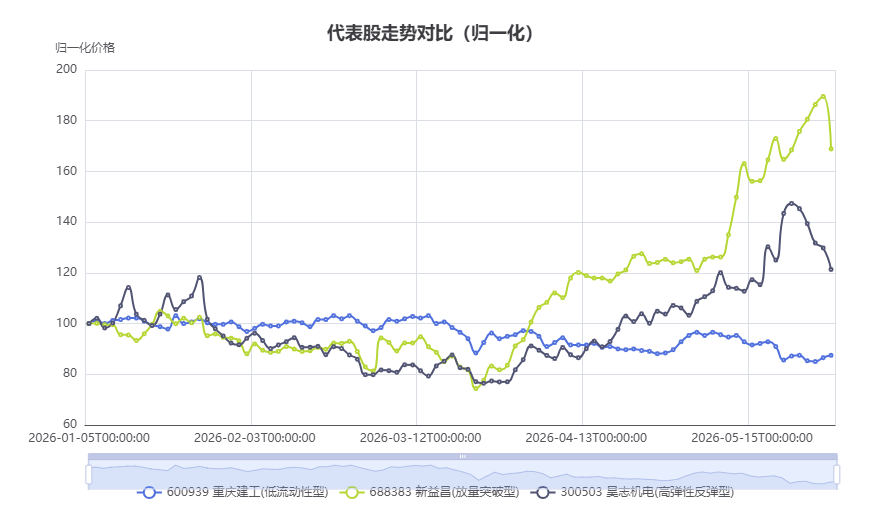
\includegraphics[width=0.95\textwidth]{13_representative_lines_cropped.png}
  \caption{三类代表股归一化走势}
  \label{fig:reprline}
\end{figure}

低流动性型代表股的价格与成交量轨迹进一步印证了类型含义。图\ref{fig:kline}将重庆建工的收盘价、5日均线、20日均线和成交量放在同一视图中，上半部分反映价格趋势，下半部分反映成交量变化。价格在3月以后出现较明显下行，短期均线多次下穿中期均线，成交量没有形成持续放大。该图与聚类画像中的低收益、低流动性特征相互印证。代表股展示的作用不在于用一只股票概括整类股票，而在于把聚类标签转化为具体时间序列观察对象，使类型含义更容易理解。

\begin{figure}[H]
  \centering
  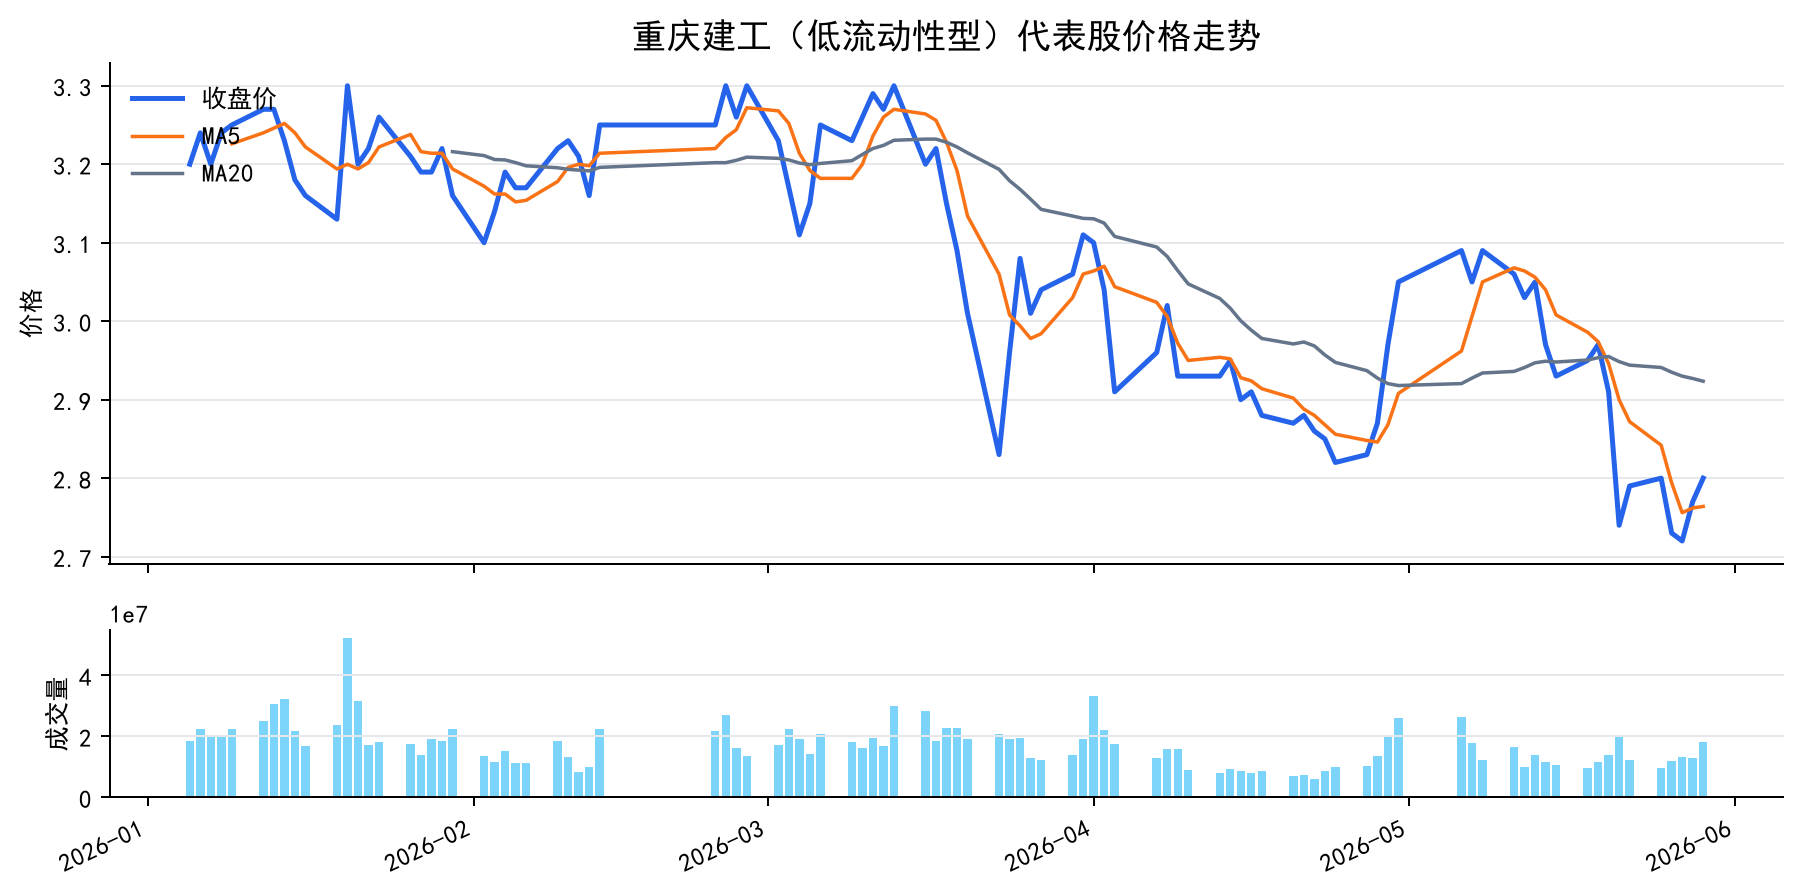
\includegraphics[width=0.88\textwidth]{14_representative_kline.png}
  \caption{重庆建工代表股价格与成交量走势}
  \label{fig:kline}
\end{figure}

\section{讨论}
中证2000样本期内的核心特征不是单一趋势，而是指数阶段性变化与个股截面分化并存。指数层面，市场先后经历抬升、回撤和修复。横截面层面，股票收益差异较大，最大回撤普遍存在，表明指数反弹并不意味着所有股票同步恢复。交易行为层面，换手率、涨跌停次数和价量相关系数显示，不同股票对资金流入、情绪变化和风险冲击的反应并不一致。

聚类画像为这种分化提供了更清晰的解释。放量突破型股票的平均收益最高，但并不以最高平均换手率为特征，表明阶段性放量、价格位置和趋势状态可能比持续活跃交易更重要。高弹性反弹型股票表现出高波动、高换手和高回撤，适合解释短期资金驱动较强的股票行为。低流动性型股票数量最多，平均收益偏弱，反映中小市值股票池中存在较大比例的低活跃度股票。若只使用指数走势作为分析依据，这些结构差异会被显著压缩。

图表选择会直接影响金融数据结论的可读性。时间序列图适合呈现市场阶段，分布图适合揭示整体离散程度，散点图适合表达双变量关系，聚类图和雷达图适合构建类型解释。不同图表承担不同分析任务，组合使用能够减少单一图表带来的误读。对于金融数据而言，图表不应只追求视觉丰富，还需要服务于证据表达。标题、坐标、图例、颜色和尺度都应与分析问题保持一致，避免因图形编码不清造成过度解释。

\section{结论}
我们基于中证2000成分股行情数据构建了面向中小市值股票画像的数据可视化分析。样本覆盖2,000只成分股和189,811条日线记录，能够支撑横截面与时间序列的联合观察。研究通过异常识别、缺失处理、特征构建、PCA 降维和 KMeans 聚类，将个股日线行情转化为收益、风险、流动性和量价行为共同构成的多维画像。指数走势、涨跌家数、成交额、小提琴图、收益排名图、风险散点图、回撤分布图、换手率散点图、价量相关分布图、PCA 聚类图、雷达图和代表股走势图共同形成了由总体市场到个体股票的分析链条。

研究结果显示，2026年1月至5月中证2000整体经历震荡上行、阶段回撤和反弹修复。个股层面的分化更为突出，放量突破型股票数量较少但平均收益最高，高弹性反弹型股票具有更高波动、更高换手和更大回撤，低流动性型股票数量最多且平均收益偏弱。由此可见，中小市值股票池的市场表现不能只通过指数判断，需要结合收益、风险、流动性和量价行为进行多维观察。数据可视化在这一过程中发挥了两方面作用，一方面把高维、密集的市场数据压缩成可阅读的图形结构，另一方面把统计特征、图表证据和分析结论放在同一证据链中，使结论更容易比较和检验。

本研究仍有进一步扩展空间。样本期仅覆盖2026年1月至5月，时间跨度较短，难以检验聚类标签在不同市场周期中的稳定性。部分基本面字段缺失，PE、PB 等指标没有充分进入图表解释。后续可以扩展更长样本期，引入行业、市值和财务指标，并结合交互式仪表盘呈现细节查询结果，使静态报告与动态探索形成互补。

\section*{参考文献}
\begin{enumerate}
  \item 中证指数有限公司。中证2000指数编制方案，2023。
  \item William S. Cleveland and Robert McGill. Graphical Perception: Theory, Experimentation, and Application to the Development of Graphical Methods. Journal of the American Statistical Association, 1984.
  \item Ben Shneiderman. The Eyes Have It: A Task by Data Type Taxonomy for Information Visualizations. IEEE Symposium on Visual Languages, 1996.
  \item Wes McKinney. pandas: a Foundational Python Library for Data Analysis and Statistics.
  \item J. D. Hunter. Matplotlib: A 2D Graphics Environment. Computing in Science and Engineering, 2007.
  \item F. Pedregosa 等。Scikit-learn: Machine Learning in Python. Journal of Machine Learning Research, 2011.
\end{enumerate}

\end{document}
